\subsection{Scan Brats18\_TCIA08\_242\_1 layer 2}
In this section we discuss the results when applying Hausdorff Distance Masks to the second extracted layer from the scan "Brats18\_TCIA08\_242\_1".


\subsubsection{Results}

\begin{figure}[H]
    \centering
    \begin{subfigure}[t]{.4\textwidth}
        \centering
        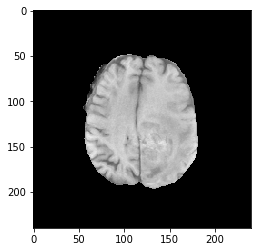
\includegraphics[width=\linewidth]{chapters/06_hdm/b_Brats18_TCIA08_242_1_L2/21.png}
        \caption{T1 modality slice}
    \end{subfigure}\hspace{1cm}%
    \begin{subfigure}[t]{.4\textwidth}
        \centering
        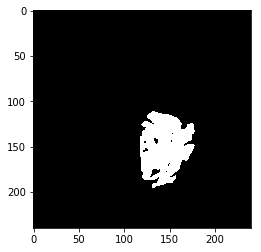
\includegraphics[width=\linewidth]{chapters/06_hdm/b_Brats18_TCIA08_242_1_L2/20.png}
        \caption{Tumor ground truth}
    \end{subfigure}
    \begin{subfigure}[t]{.45\textwidth}
        \centering
        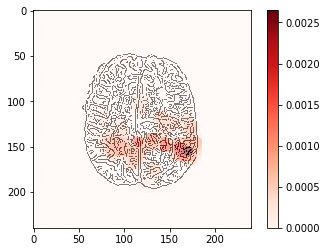
\includegraphics[width=\linewidth]{chapters/06_hdm/b_Brats18_TCIA08_242_1_L2/23.png}
        \caption{Regions where the applied masks reduce the accuracy of the segmentation}
    \end{subfigure}\hspace{1cm}%
    \begin{subfigure}[t]{.45\textwidth}
        \centering
        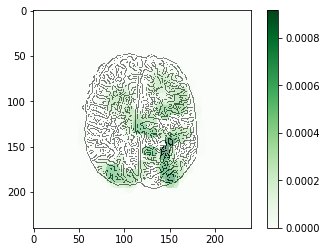
\includegraphics[width=\linewidth]{chapters/06_hdm/b_Brats18_TCIA08_242_1_L2/24.png}
        \caption{Regions where the applied masks increase the accuracy of the segmentation}
    \end{subfigure}
    \caption{Modality T1 analyzed with Hausdorff Distance Masks. The image (c) shows regions which match the tumor, but also shows regions outside of the tumor which influence the segmentation. Image (d) which shows accuracy increases when occluded shows regions in almost the whole brain.}
    \label{brats_tcia08_t1}
\end{figure}


\begin{figure}[H]
    \centering
    \begin{subfigure}[t]{.4\textwidth}
        \centering
        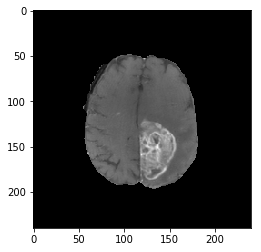
\includegraphics[width=\linewidth]{chapters/06_hdm/b_Brats18_TCIA08_242_1_L2/26.png}
        \caption{T1 contrast enhanced modality slice}
    \end{subfigure}\hspace{1cm}%
    \begin{subfigure}[t]{.4\textwidth}
        \centering
        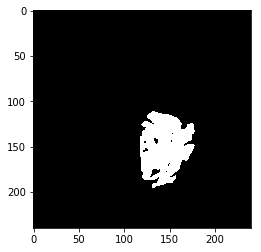
\includegraphics[width=\linewidth]{chapters/06_hdm/b_Brats18_TCIA08_242_1_L2/25.png}
        \caption{Tumor ground truth}
    \end{subfigure}
    \begin{subfigure}[t]{.45\textwidth}
        \centering
        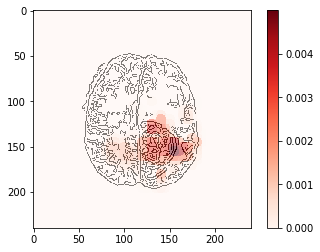
\includegraphics[width=\linewidth]{chapters/06_hdm/b_Brats18_TCIA08_242_1_L2/28.png}
        \caption{Regions where the applied masks reduce the accuracy of the segmentation}
    \end{subfigure}\hspace{1cm}%
    \begin{subfigure}[t]{.45\textwidth}
        \centering
        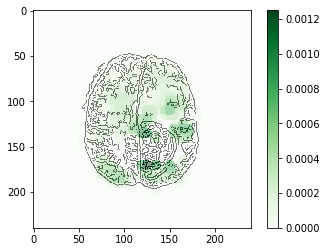
\includegraphics[width=\linewidth]{chapters/06_hdm/b_Brats18_TCIA08_242_1_L2/29.png}
        \caption{Regions where the applied masks increase the accuracy of the segmentation}
    \end{subfigure}
    \caption{Modality T1 contrast enhanced analyzed with Hausdorff Distance Masks. The important regions which decrease the accuracy of the segmentation are located in the tumor region which are clearly visible in this contrast enhanced scan modality.}
    \label{brats_tcia08_t1ce}
\end{figure}

\begin{figure}[H]
    \centering
    \begin{subfigure}[t]{.4\textwidth}
        \centering
        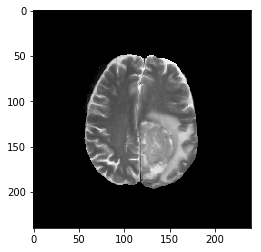
\includegraphics[width=\linewidth]{chapters/06_hdm/b_Brats18_TCIA08_242_1_L2/31.png}
        \caption{T2 modality slice}
    \end{subfigure}\hspace{1cm}%
    \begin{subfigure}[t]{.4\textwidth}
        \centering
        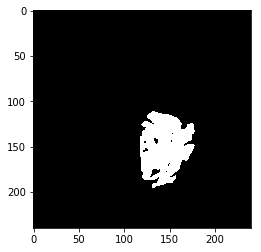
\includegraphics[width=\linewidth]{chapters/06_hdm/b_Brats18_TCIA08_242_1_L2/30.png}
        \caption{Tumor ground truth}
    \end{subfigure}
    \begin{subfigure}[t]{.45\textwidth}
        \centering
        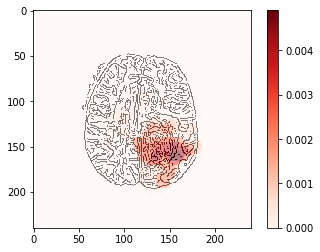
\includegraphics[width=\linewidth]{chapters/06_hdm/b_Brats18_TCIA08_242_1_L2/33.png}
        \caption{Regions where the applied masks reduce the accuracy of the segmentation}
    \end{subfigure}\hspace{1cm}%
    \begin{subfigure}[t]{.45\textwidth}
        \centering
        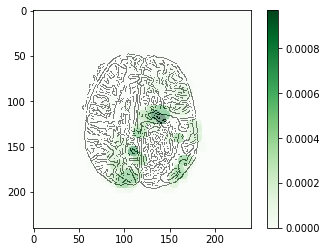
\includegraphics[width=\linewidth]{chapters/06_hdm/b_Brats18_TCIA08_242_1_L2/34.png}
        \caption{Regions where the applied masks increase the accuracy of the segmentation}
    \end{subfigure}
    \caption{Modality T2 analyzed with Hausdorff Distance Masks. The regions decreasing the accuracy when occluded (image (c)) are in the tumor center which is visible in this modality. Regions increasing the accuracy when occluded (d) are around the tumor borders.}
    \label{brats_tcia08_t2}
\end{figure}

\begin{figure}[H]
    \centering
    \begin{subfigure}[t]{.4\textwidth}
        \centering
        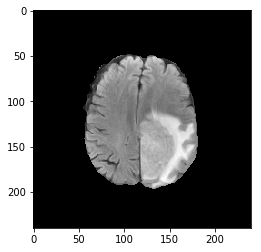
\includegraphics[width=\linewidth]{chapters/06_hdm/b_Brats18_TCIA08_242_1_L2/36.png}
        \caption{FLAIR modality slice}
    \end{subfigure}\hspace{1cm}%
    \begin{subfigure}[t]{.4\textwidth}
        \centering
        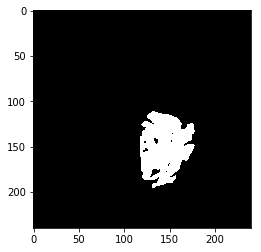
\includegraphics[width=\linewidth]{chapters/06_hdm/b_Brats18_TCIA08_242_1_L2/35.png}
        \caption{Tumor ground truth}
    \end{subfigure}
    \begin{subfigure}[t]{.45\textwidth}
        \centering
        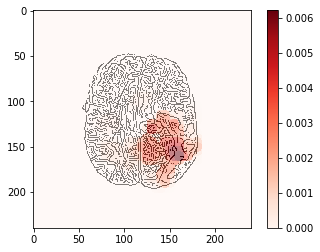
\includegraphics[width=\linewidth]{chapters/06_hdm/b_Brats18_TCIA08_242_1_L2/38.png}
        \caption{Regions where the applied masks reduce the accuracy of the segmentation}
    \end{subfigure}\hspace{1cm}%
    \begin{subfigure}[t]{.45\textwidth}
        \centering
        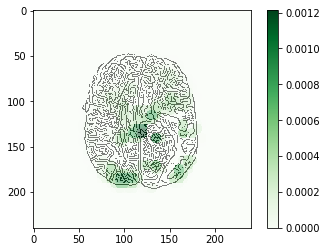
\includegraphics[width=\linewidth]{chapters/06_hdm/b_Brats18_TCIA08_242_1_L2/39.png}
        \caption{Regions where the applied masks increase the accuracy of the segmentation}
    \end{subfigure}
    \caption{Modality FLAIR analyzed with Hausdorff Distance Masks. The region marked to decreasing the accuracy when occluded (image (c)) is quite big, as is expected from the FLAIR modality which shows a big part of the tumor.}
    \label{brats_tcia08_flair}
\end{figure}

\subsubsection{Discussion}
Figures \ref{brats_tcia08_t1}, \ref{brats_tcia08_t1ce}, \ref{brats_tcia08_t2} and \ref{brats_tcia08_flair} show HDM results applied on all four modalities. The generated visualizations for regions decreasing the accuracy look very similar, mostly matching the parts of the tumor that is visible on the corresponding modality. The T1 modality seems to have the smallest impact on the generated segmentation, the maximal deviation from the baseline distance is only 0.0025 compared to 0.005 for T1 contrast enhanced and T2. FLAIR is highest with a deviation of 0.006.